\newpage
\section{Eksamensopgave 5 - Kinematik}
\begin{figure}[h!]
    \centering
    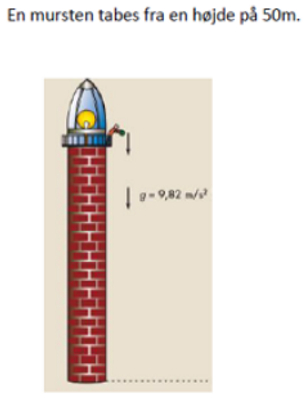
\includegraphics[width=0.3\textwidth]{figures/kinematik.png}
    \caption{Kimenatik opgave}
\end{figure}

\subsection{Beregn murstenens position efter 0,1s}
Først start med at identificer de kendte værdier:
\\\\
Startposition: 50 meter \newline
Start hastighed: 0 m/s (da den falder frit fra hvile position)\newline
Tid: 0,1 sekunder \newline
Tyngdeacceleration: \begin{math}9,82m/s^{2}\end{math}


\subsubsection{Brug den kinematiske formel for position}
Den generelle formel for position ved frit fald er:
\begin{equation*}
    s= \frac{1}{2} \cdot g \cdot t^{2}
\end{equation*}
s = strækning\newline
g = Tyngdeacceleration\newline
t = tid

\subsubsection{Indsæt værdierne i formlen og udregn}
\begin{equation*}
    \frac{1}{2} \cdot 9,82 \frac{m}{s^{2}}\cdot (0,1 \cdot s)^{2}= 0,04910m \approx \mathcolorbox{yellow}{0,049m}
\end{equation*}
Murstenens position efter 0,1s er $49,95m$

\subsection{Bestem hvor lang tid der går, inden murstenen rammer jorden}

Først identificer vi de kendte værdier som er brugt ovenover

\subsubsection{Brug den kinematiske formel for position}
For at finde tiden det tager for murstenen at ramme jorden, bruger vi formlen for position ved frit fald.
\begin{equation*}
    \frac{1}{2}\cdot g\cdot t^{2}=s
\end{equation*}

Multiplicer begge sider med 2:
\[ g \cdot t^2 = 2s \]

Divider begge sider med \( g \):
\[ t^2 = \frac{2s}{g} \]

Tag kvadratroden af begge sider:
\[ t = \sqrt{\frac{2s}{g}} \]
Indsæt værdierne i formlen og udregn nu: 
\begin{equation*}
    t = \sqrt{\frac{2 \cdot 50m}{9,82m/s^2}} = 3,191 s \approx \mathcolorbox{yellow}{3,2s}
\end{equation*}
Da det laveste antal betyende cifere er to angives resultatet i to betyende cifere. Derfor giver t = 3,2s. Hvilket betyder at der går cirka 3,2s før murstenen rammer jorden.

\subsection{Beregn murstenens hastighed, lige inden den rammer jorden}
For at kunne udregne dett bruger vi formlen nedenunder.
\begin{equation*}
    v=a\cdot t
\end{equation*}
v = velocity\newline
a = acceleration\newline
t = tid
\subsubsection{Indsæt de kendte værdier}
\begin{equation*}
    9,82 \frac{m}{s^{2}}\cdot 3,191s = \mathcolorbox{yellow}{31,34 m/s}
\end{equation*}


\newpage